\documentclass{article}

% Language setting
% Replace `english' with e.g. `spanish' to change the document language
\usepackage[polish]{babel}

% Set page size and margins
% Replace `letterpaper' with `a4paper' for UK/EU standard size
\usepackage[a4paper,top=2cm,bottom=2cm,left=3cm,right=3cm,marginparwidth=1.75cm]{geometry}

% Useful packages
\usepackage{polski}
\usepackage[utf8]{inputenc}
\usepackage{amsmath}
\usepackage{graphicx}
\usepackage[colorlinks=true, allcolors=blue,unicode]{hyperref}
\usepackage{courier}
\usepackage[T1]{fontenc}
\usepackage{lastpage}

\usepackage{fancyhdr}
\pagestyle{fancy}
\fancyhead[L]{Specyfikacja funkcjonalna}
\fancyhead[C]{}
\fancyhead[R]{Kamil Fryszkowski, Oskar Biwejnis}
\cfoot{\thepage/\pageref{LastPage}}


\title{Specyfikacja funkcjonalna projektu w języku Java}
\author{Kamil Fryszkowski, Oskar Biwejnis}


\begin{document}
\maketitle
\thispagestyle{fancy}

\section{Cel projektu}
Celem projektu jest stworzenie graficznej aplikacji, której główną funkcjonalnością jest rozwiązanie problemu znajdowania najkrótszej ścieżki w grafie ważonym skierowanym.
Zrobione to zostanie poprzez stworzenie programu w języku Java, który wykorzysta do tego algorytm Dijkstry i jednocześnie spełnia następujące założenia:
\begin{itemize}
\item Potrafi wygenerować graf, w zależności od podanych parametrów
\item Zapisuje wygenerowany graf do pliku o określonym formacie:
\begin{itemize}
\item W pierwszej linii podane są dwie liczby całkowite m i n, które określają kolejno liczbę kolumn i wierszy grafu
\item Kolejne wiersze pokazują dostępne krawędzie. K-ty wiersz pliku (dla K > 1) określa wszystkie wierzchołki, do których można przejść z wiersza K-2 i ich wagi

\item Pierwszy wiersz określa m=7 jako liczbę wierszy i n=4 jako liczbę kolumn grafu.
\item Drugi wiersz określa możliwe połączenia dla wierzchołka K – 2 = 0 (K = 2). Oznacza, że koszt przejścia z wierzchołka 0 do wierzchołka 1 wynosi 0.8864… i koszt przejścia z wierzchołka 0 do 4 wynosi 0.2187….
\item Trzeci wiersz określa możliwe połączenia dla wierzchołka K – 2 = 1 (K = 3). Oznacza to, że koszt przejścia z wierzchołka 1 do wierzchołka 5 wynosi 0.2637… i tak dalej.\\
\\
Przykład pliku: \\\\
\texttt{\footnotesize 7 4\\
	 1 :0.8864916775696521  4 :0.2187532451857941 \\
	 5 :0.2637754478952221  2 :0.6445273453144537  0 :0.4630166785185348 \\
	 6 :0.8650384424149676  3 :0.42932761976709255  1 :0.6024952385895536 \\
     ...\\}
\end{itemize}
\item Z takiego samego formatu potrafi odczytać graf
\item Sprawdza czy graf jest spójny przy pomocy algorytmu BFS
\item Posiada przystępny interfejs graficzny, pozwalający użytkownikowi na wygodne korzystanie z programu
\end{itemize}

Struktura grafów używanych przez program przypomina kratkę z zeszytu szkolnego, gdzie krawędziami są linie pionowe i poziome, a na ich przecięciach znajdują się wierzchołki. (Rysunek \ref{fig:graf}.)\\\\\\\\\\\\\\\\\\

\begin{figure}[h]
\centering
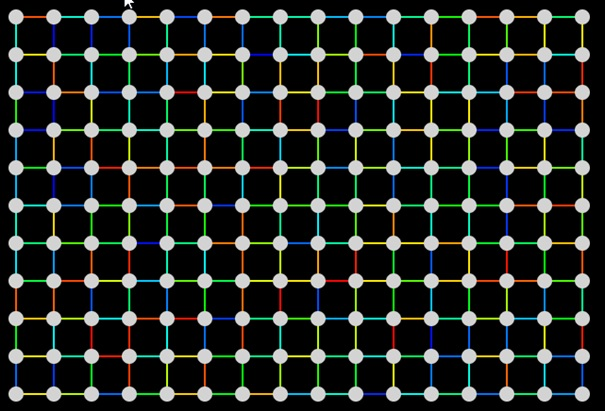
\includegraphics[width=0.5\textwidth]{grafik.jpg}
\caption{\label{fig:graf}Graficzna reprezentacja przykładowego grafu. (Źródło: materiały z ISOD)}
\end{figure}

\section{Opis działania programu i graficznego interfejsu użytkownika}

\begin{figure}[h]
\centering
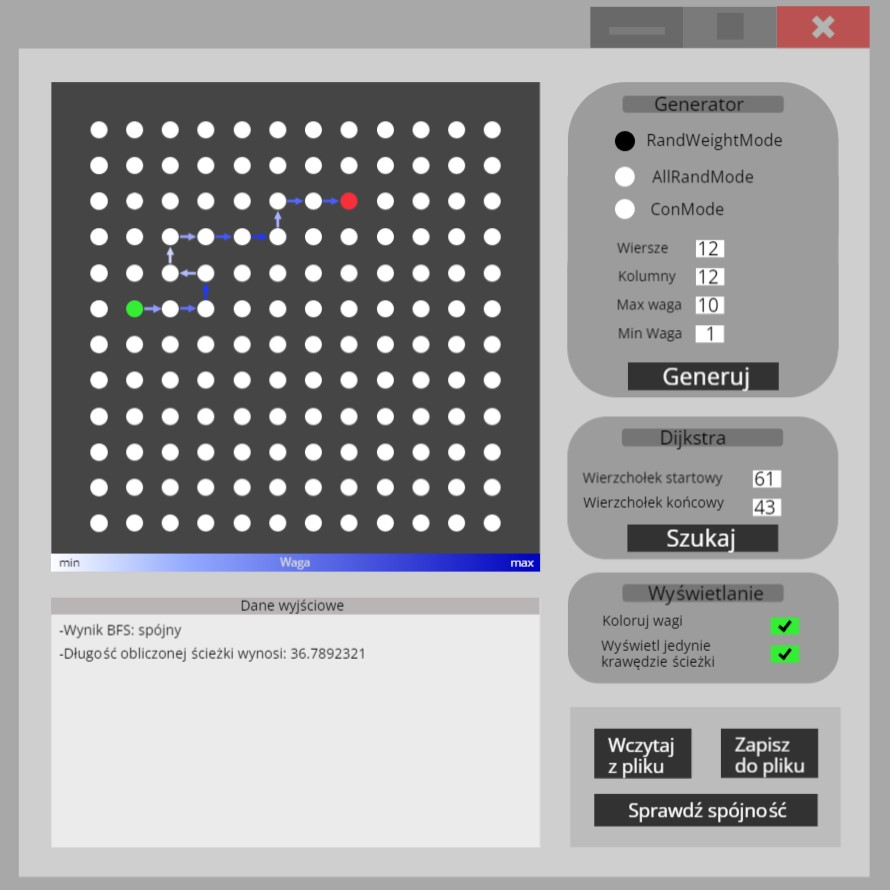
\includegraphics[width=0.8\textwidth]{gui3.jpg}
\caption{\label{fig:gui}Projekt GUI w okienku o stałym rozmiarze 700x700px (Źródło: opracowanie własne)}
\end{figure}

\paragraph{Poszczególne elementy graficznego interfejsu użytkownika:}
\begin{itemize}
\item Wyświetlanie Grafu\\\\
Z lewej strony wyświetla się wygenerowany lub wczytany z pliku graf, którego wielkość jest skalowana aby dopasować się do rozmiaru podokienka (maksymalna wielkość dla poprawnego działania: 75x75) Graf może zawierać pokolorowane krawędzie w zależności od ich wagi (im większa waga tym ciemniejszy kolor). Można również wyłączyć wyświetlanie wszystkich krawędzi, aby pokazać jedynie trasę między startowym a końcowym wierchołkiem, między którymi szukana jest ścieżka.\\
\item Generator\\\\
Generator pozwala wybrać jeden z trzech trybów pracy:
\begin{itemize}
    \item RandWeightMode - pozwala na stworzenie grafu, w którym istnieją wszystkie krawędzie zawierające się w danym przedziale wierzy i kolumn z wygenerowanymi losowo z danego przedziału wagami
    \item AllRandMode - pozwala na stworzenie grafu, w którym istnieje jedynie określona szansa na powstanie danej krawędzi
    \item ConMode - działa jak AllRandMode, jednak graf generuje się tak długo, aż nie będzie spójny.
\end{itemize}
Do danych trybów pracy należy dobrać również parametry znajdujące się poniżej trybu w GUI: wiersze (domyślnie 10), kolumny (domyślnie 10), max waga (domyślnie 1), min waga (domyślnie 0).\\

\item Dijkstra\\\\
Kiedy wygenerowany lub wczytany graf pojawi się z lewej strony okna, program pozwoli na znalezienie ścieżki między dwoma punktami, która wyświetli się na schemacie grafu, a jej długość oraz diagram pojawi się poniżej niego\\

\item Obsługa pliku\\\\
Każdy wygenerowany graf można zapisać do pliku przy pomocy opcji "Zapisz". Można również wczytać wygenerowany wcześniej graf przy pomocy opcji "Wczytaj".
\item Sprawdzanie spójności\\\\
Program za pomocą algorytmu BFS sprawdzi spójność grafu i  następnie wypisze wynik w terminalu
\end{itemize}


\section{Obsługa błędów}
\paragraph{Możliwe błędy przy uruchamianiu programu:}

\begin{itemize}

\item \texttt{Argument nie jest liczbą, lub zawiera się poza określonym zakresem} \\ 
Ten błąd pojawia się, kiedy jeden z argumentów, który powinien być liczbą (kolumny, wiersze, dolny zakres wag, górny zakres wag, pary punktów), nią nie jest lub przekracza zakres w którym działa program

\item \texttt{Nie udało się otworzyć pliku} \\
Ten błąd pojawia się, kiedy nie można uzyskać dostępu do pliku z grafem 

\item \texttt{Nie udało się utworzyć pliku} \\
Ten błąd pojawia się, kiedy nie można było stworzyć pliku z wygenerowanym grafem

\item \texttt{Niewystarczająca liczba argumentów } \\
Ten błąd pojawia się, kiedy podana zostanie niewystarczająca liczba argumentów

\end{itemize}

\end{document}